\section{Security considerations}
In order to increase security in our system, different considerations was made. These considerations are made in order to make it more difficult for outsiders to access the system as well hide sensitive user information except for the mac-address.

\subsection*{HTTPS and Certificates} 
%  HTTPS and SSL certificate. May want to talk more about where we could use it in our system
To increase security against unauthorised personal a HTTPS connection could be established. HTTPS is short for \textit{Hyper Text Transfer Protocol Secure} and is the secure form of HTTP. With HTTP everything send as plain text and can be read by anyone who access the connection, but what makes HTTPS secure is that this pure text is encrypted. This means that if someone gains access the connection they would not be able to read the information. A secure connection is therefore very important on sites that handles sensitive information such as CPR-numbers or credit card information and this can be achieved by using HTTPS\cite{HTTPS}.

\begin{figure}[ht]
	\begin{center}
		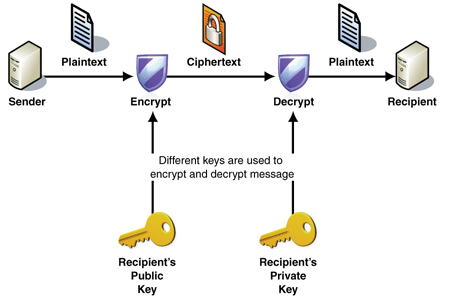
\includegraphics[scale=0.9]{graphics/HTTPS.png}
		\caption{HTTPS \cite{https_pic}.}
		\label{fig:HTTPS}
	\end{center} 
\end{figure}

\Cref{fig:HTTPS} shows how HTTPS works after the key exchange have taken place. First the sender sends plain text, which is encrypted using the recipients public key. The encrypted message is then send and decrypted using the recipients private key before plain text is received.

The handshake between the browser and a site using HTTPS starts with an exchange of public SSL-keys (Secure Socket Layer). The SSL-key is unique and enable encrypt of the data you send, the encrypted data can then only be decrypted with your own private key\cite{HTTPS}. 

\subsection*{Hash passwords}
\subsection*{Adding servers to client}
\subsection*{Accessors}
\subsection*{Hard-coded passwords}

\subsection*{Visibility}
As of now the most of our system is public, by decreasing the level of visibility to have more private and protected classes and methods, the system would be more secure.
 
\subsection*{Obfuscate personal information}
In order to ensure our users personal information, it have been considered to obfuscate their E-mail as well as their Ip-addresses in the same manner as it is done to the MAC-address. By doing so there will be no way for outsiders to identify people unwilling to have their information stored.
